\documentclass[xcolor=svgnames]{beamer}
\mode<presentation>
{
      \setbeamertemplate{footline}[page number]
      \setbeamercovered{transparent}
      \setbeamertemplate{navigation symbols}{}
      \usecolortheme[named=DarkGreen]{structure}
}

\usepackage[english]{babel}
\usepackage{times}
\usepackage{url}
\usepackage{CJKutf8}
\usepackage{graphics}
\usepackage{amsmath}
\usepackage{listings}
\lstset{breakatwhitespace,
language=C,
columns=fullflexible,
keepspaces,
breaklines,
tabsize=3,
showstringspaces=false,
extendedchars=true}

\begin{document}
\begin{CJK*}{UTF8}{gbsn}


\title{操作系统期末复习提纲}

\begin{frame}
\maketitle
\end{frame}

\begin{frame}{操作系统中三个最重要的概念}
\begin{enumerate}
\item 把处理器CPU抽象为\alert{进程}
\item[]
\item 把物理内存抽象为虚拟内存和虚拟\alert{地址空间}
\item[]
\item 把永久存储介质(如硬盘)抽象为\alert{文件}
\end{enumerate}
\end{frame}

\begin{frame}{操作系统中三个最重要的概念}
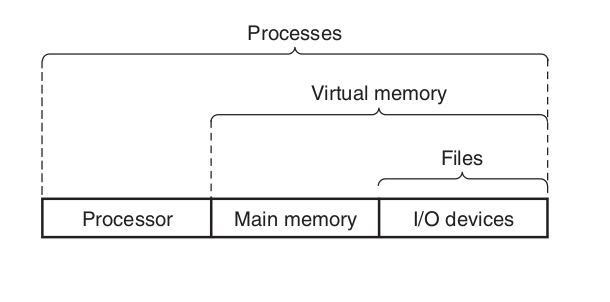
\includegraphics[width=1.0\textwidth]{osabstractions.png}
\end{frame}

\begin{frame}{文件的属性}
\begin{itemize}
\item protection
\item password
\item creator
\item owner
\item read-only flag
\item lock flag
\item creation time
\item time of last access
\item current size
\end{itemize}
\end{frame}

\begin{frame}{文件的实现: 连续存储方式}
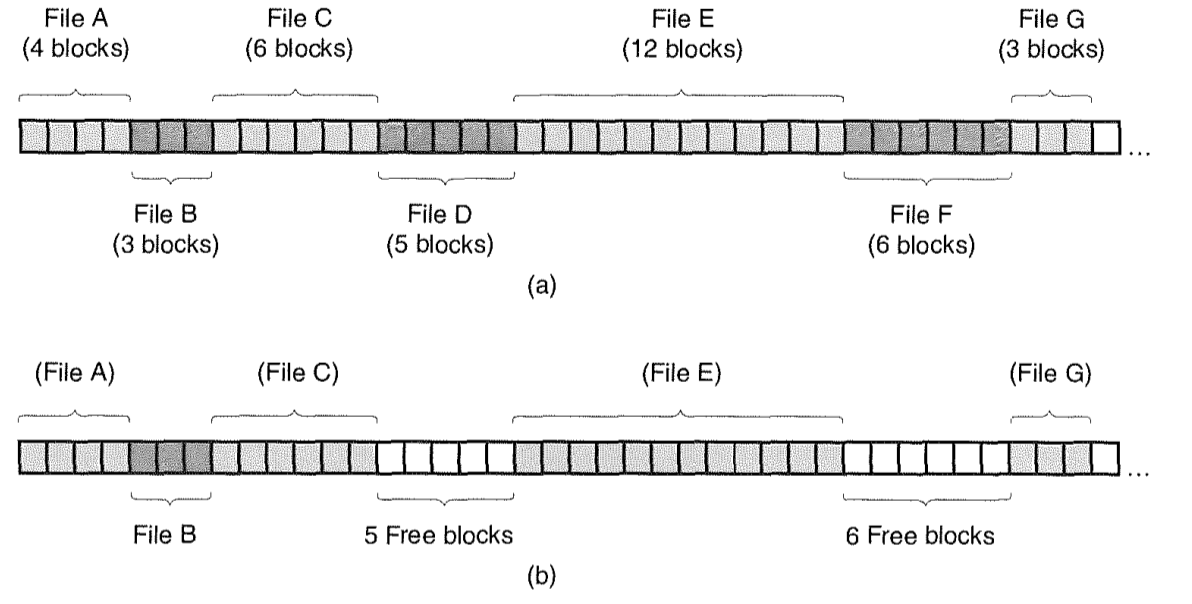
\includegraphics[width=1.0\textwidth]{cont.png}
\end{frame}

\begin{frame}{文件的实现: 连续存储方式}
%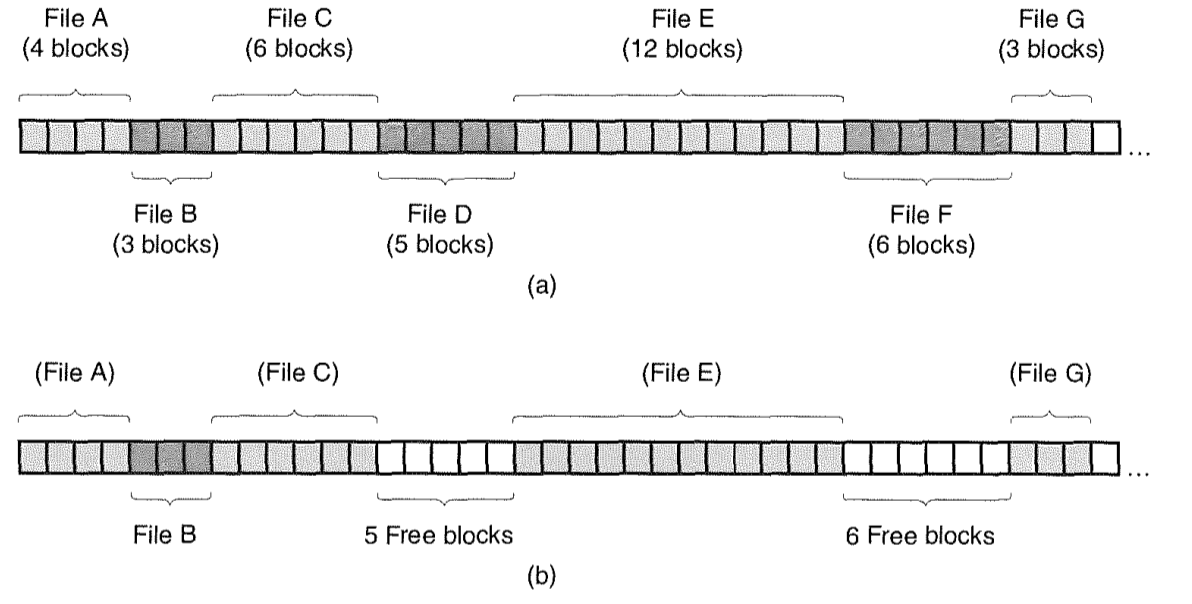
\includegraphics[width=1.0\textwidth]{cont.png}
连续存储方式有两个重要优点:
\begin{itemize}
\item 实现容易:只需记录每个文件在磁盘上起始块地址,以及所占的总块数
\item 读写速度非常块:每次读写仅需1次机械移动寻址过程
\end{itemize}

\alert{缺点?} --- 容易导致文件系统大量碎片(前图)

\alert{应用?} --- CD-ROM上的文件系统, why?
\end{frame}

\begin{frame}{文件的实现: 线性链表存储方式}
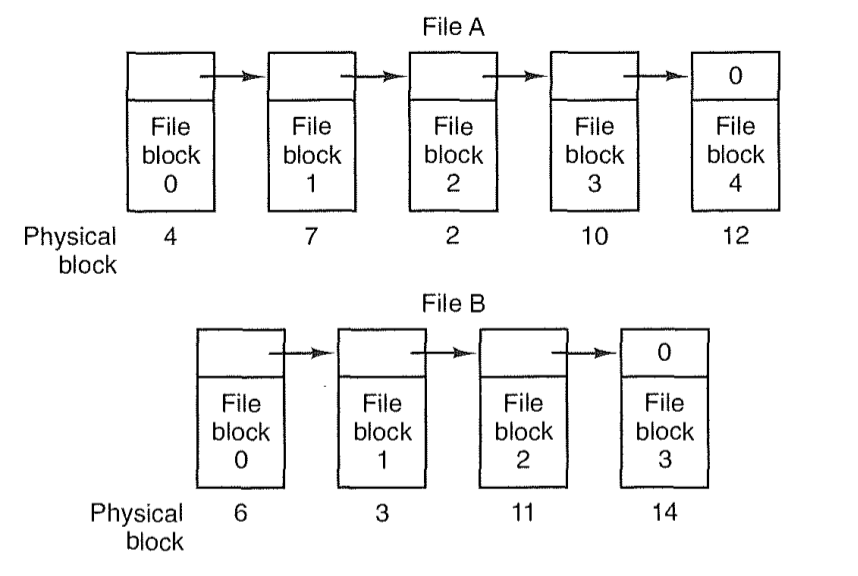
\includegraphics[width=1.0\textwidth]{linked.png}

\alert{注}: 每个磁盘块的前几个字节用于记录存储该文件的下一个磁盘块地址
\end{frame}

\begin{frame}{文件的实现: 线性链表存储方式}
线性链表存储方式的优点:
\begin{itemize}
\item 只需记录每个文件在磁盘上的起始地址
\item 避免碎片问题
\end{itemize}

缺点:不利于随机访问, why?
\end{frame}

\begin{frame}{文件的实现: I-nodes}
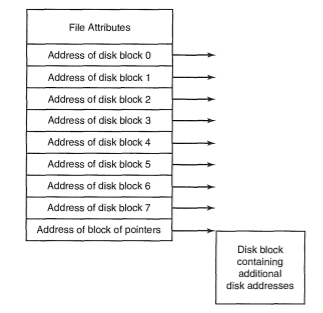
\includegraphics[width=0.8\textwidth]{inodes.png}
\end{frame}

\begin{frame}{文件的实现: I-nodes}
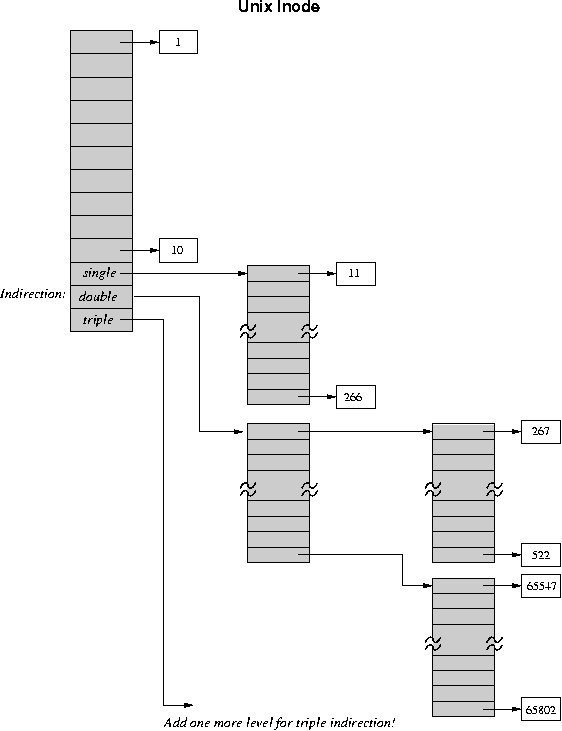
\includegraphics[width=0.6\textwidth]{inode22.png}
\end{frame}

\begin{frame}{文件系统的布局}
考虑磁盘上的文件系统:
\begin{itemize}
\item 磁盘可以进行分区,用磁盘分区表记录每个分区的边界
\item 第0扇区:MBR(Master Boot Record, 主引导记录), 存放引导程序及磁盘分区表
\item MBR中的引导程序选择某个分区中的操作系统进行引导
\item 每个分区中有一个磁盘块用于启动该分区上的操作系统(boot block)
\item 超级块(superblock): 存放该分区上的文件系统参数(类型、块数等信息)
\end{itemize}
\end{frame}

\begin{frame}{文件系统的布局}
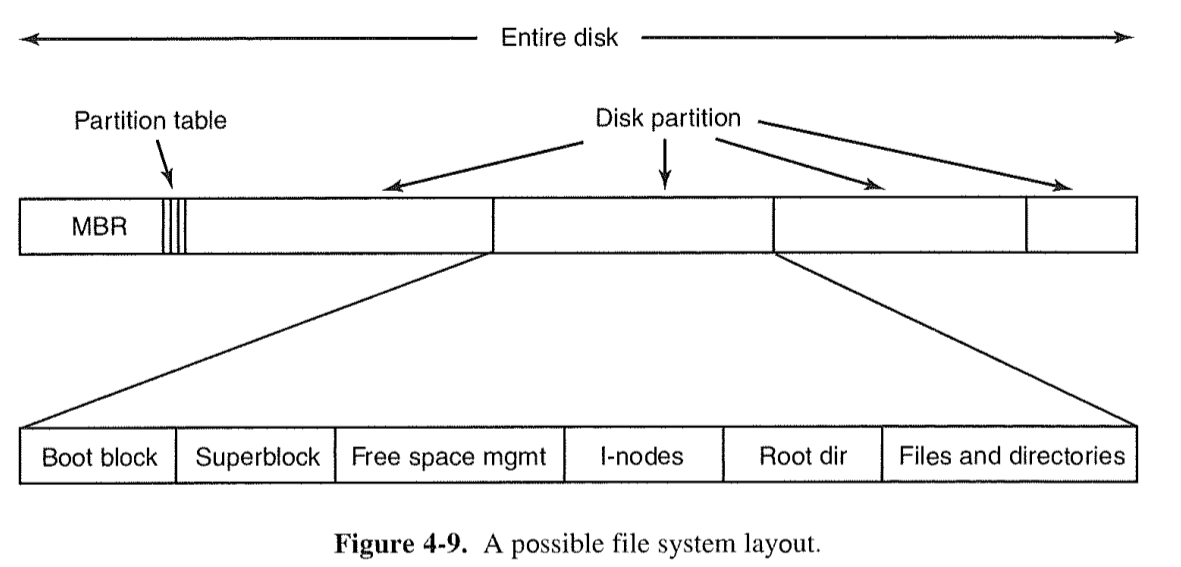
\includegraphics[width=1.0\textwidth]{layout.png}
\end{frame}

\begin{frame}[fragile]
\frametitle{Linux内核与普通应用程序的区别}
\begin{itemize}
\item 内核不能使用C语言标注库函数(及C标准头文件)
\item Linux内核编程使用的是GNU C而不是标准C语言
\item 内核代码缺乏内存保护机制(应用程序则有)
%\item 内核无法方便地使用浮点数操作指令
\item 与应用程序比,内核运行时的栈非常小
\item 内核代码必须正确处理同步与并发问题
\item 可移植性对内核而言非常重要
\end{itemize}
\end{frame}

\begin{frame}[fragile]
\frametitle{为什么内核不能使用C语言库函数及头文件?}
\begin{block}{原因}
\begin{itemize}
\item chicken-and-egg问题
\item C标准库对内核而言太庞大、低效
\end{itemize}
\end{block}
\begin{block}{Linux内核的应对策略}
\begin{itemize}
\item 自己实现部分库函数功能:\verb|lib/string.c|,对应头文件\verb|<linux/string.h>|
\item 标准库中printf函数在内核中对应的是printk
\begin{itemize}
\item 例如 \verb|printk(KERN_ERR "this is an error!\n")|
\end{itemize}
\end{itemize}
\end{block}
\end{frame}

\defverbatim[colored]\lstlisthead{
\begin{lstlisting}[tabsize=8,basicstyle=\ttfamily]
struct list_head {
    struct list_head *next, *prev;
};
\end{lstlisting}
}
\defverbatim[colored]\lstlistheadusage{
\begin{lstlisting}[tabsize=8,basicstyle=\ttfamily]
struct task_struct {
    ...
    struct list_head run_list;
    ...
};
\end{lstlisting}
}
\begin{frame}[fragile]
\frametitle{list\_head的定义}
\begin{block}{include/linux/list.h}
\lstlisthead
\end{block}
\begin{block}{思考}
这种只有指针而没有数据的list\_head能有什么用处?
\end{block}
\end{frame}

\begin{frame}[fragile]
\frametitle{list\_head的使用方法举例}
\begin{block}{include/linux/sched.h}
\lstlistheadusage
\end{block}
\begin{block}{思考}
与fox结构相比,使用list\_head构造链表有什么好处?
\end{block}
\end{frame}

\defverbatim[colored]\lstinit{
\begin{lstlisting}[tabsize=8,basicstyle=\ttfamily]
#define LIST_HEAD_INIT(name) \
        { &(name), &(name) }

#define LIST_HEAD(name) \
    struct list_head name = LIST_HEAD_INIT(name)
\end{lstlisting}
}
\begin{frame}[fragile]
\frametitle{list\_head结构的静态初始化}
\begin{block}{include/linux/list.h}
\lstinit
\end{block}
\begin{block}{LIST\_HEAD的使用方法}
%\lstinit
例: \verb|LIST_HEAD(packet_list)|声明一个名为\verb|packet_list|的表头变量并将其初始化为空表。
\end{block}
\end{frame}

\begin{frame}[fragile]
\frametitle{针对list结构的操作}
\begin{itemize}
\item \verb|list_add(new, head)| 把new插入head后面
\item \verb|list_add_tail(new, head)| 把new插入head前面
\item \verb|list_del(entry)| 把entry从链表中删除
\item \verb|list_empty(head)| 判断链表head是否为空
\item \verb|list_splice(list, head)| 合并list和head
\item \verb|list_for_each(pos, head)| 遍历以head为头的链表
\end{itemize}
\end{frame}

\defverbatim[colored]\lstforeach{
\begin{lstlisting}[tabsize=8,basicstyle=\ttfamily]
struct list_head *p;

list_for_each(p, &list) {
    if (!condition) continue;
    return list_entry(p, struct task_struct, 
                      run_list);
}

return NULL;
\end{lstlisting}
}
\begin{frame}[fragile]
\frametitle{针对list结构的操作举例: list\_for\_each}
\lstforeach
\end{frame}

\defverbatim[colored]\lsthlist{
\begin{lstlisting}[tabsize=8,basicstyle=\ttfamily]
struct hlist_head {
    struct hlist_node *first;
};

struct hlist_node {
    struct hlist_node *next, **pprev;
};
\end{lstlisting}
}
\begin{frame}[fragile]
\frametitle{实现哈希表: hlist\_head与hlist\_node}
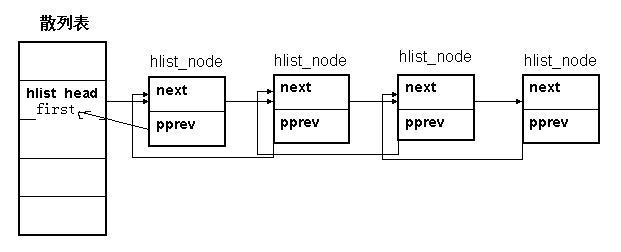
\includegraphics[width=0.9\textwidth]{hlist.jpeg}
\begin{block}{include/linux/list.h}
\lsthlist
\end{block}
\end{frame}

\begin{frame}[fragile]
\frametitle{针对hlist\_head与hlist\_node的操作}
\begin{itemize}
\item \verb|hlist_add_head|
\item \verb|hlist_add_before|
\item \verb|hlist_add_after|
\item \verb|hlist_del(entry)|
\item \verb|hlist_empty(head)| 
\end{itemize}
\end{frame}

\begin{frame}[fragile]
\frametitle{Linux内核关键数据结构:hlist\_head与hlist\_node}
\begin{block}{思考及课外练习}
%阅读include/linux/list.h中
%\verb|hlist_add_head()|, \verb|hlist_del()|, \verb|hlist_empty()|, \verb|hlist_add_before()|等函数的实现,思考:
%
\begin{enumerate}
\item \verb|hlist_node|中的\verb|pprev|字段指向什么内容?
%\item 为什么\verb|pprev|采用二重指针?
\item 为什么\verb|hlist_head|中只有一个成员\verb|first|?
\item \verb|hlist_head|可否直接用\verb|hlist_node|代替?
\end{enumerate}
\end{block}
\end{frame}

\defverbatim[colored]\lstpidmax{
\begin{lstlisting}[tabsize=8,basicstyle=\ttfamily]
/*
 * This controls the default maximum pid 
 *   allocated to a process
 */
#define PID_MAX_DEFAULT 0x8000
\end{lstlisting}
}
\begin{frame}{Linux区别进程的方式: pid字段}
%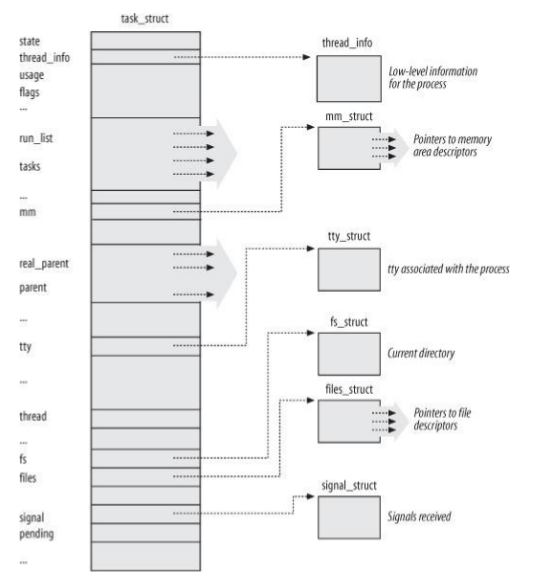
\includegraphics[width=0.7\textwidth]{taskstruct.png}
\begin{itemize}
\item 在内核中,对进程的各种操作均通过task\_struct实现
\item 用户角度,每个进程有唯一编号(PID). 进程的PID保存于task\_struct的pid字段中。
\begin{itemize}
\item 例如:kill()系统调用的参数为PID
\item 内核需要快速从PID找到对应的task\_struct进行操作(后面讲具体方法)
\end{itemize}
\end{itemize}
\begin{block}{PID可取的最大值: include/linux/threads.h}
\lstpidmax
\end{block}
\end{frame}

\begin{frame}{Linux区别进程的方式: pid字段}
\begin{block}{思考}
\begin{enumerate}
\item 为什么要限制PID可取的最大值?
\item[]
\item 如果系统中进程个数超过这个最大值怎么办?
\end{enumerate}
\end{block}
\end{frame}

\defverbatim[colored]\lsttasks{
\begin{lstlisting}[tabsize=8,basicstyle=\ttfamily]
struct task_struct {
    ...
    struct list_head tasks;
    ...
};
\end{lstlisting}
}

\begin{frame}{内核遍历所有进程的方式: tasks字段}
\begin{block}{task\_struct中的tasks字段:将系统中所有进程连接起来} 
\lsttasks
\end{block}
\begin{block}{系统中所有进程组成的链表}
%\lststates
以init\_task为表头,进程描述符的tasks字段将所有进程连接起来
\end{block}
\begin{block}{遍历系统中所有进程的宏: for\_each\_process}
阅读并理解include/linux/sched.h中for\_each\_process的实现。
\end{block}
\end{frame}

\defverbatim[colored]\lstrunning{
\begin{lstlisting}[tabsize=8,basicstyle=\ttfamily]
struct task_struct {
    ...
    int prio, static_prio;
    struct list_head run_list;
    prio_array_t *array;
    ...
};
\end{lstlisting}
}
\begin{frame}%{Linux进程描述符: Process Descriptor}
\frametitle{与进程调度相关的字段}
\lstrunning
\begin{block}{各字段的含义}
\begin{itemize}
\item prio 为进程当前优先级 (0 -- 139)
\item run\_list 用于连接所有相同优先级的进程
\item array?
\end{itemize}
\end{block}
\end{frame}

\defverbatim[colored]\lstprio{
\begin{lstlisting}[tabsize=8,basicstyle=\ttfamily]
struct prio_array {
    unsigned int nr_active;
    unsigned long bitmap[BITMAP_SIZE];
    struct list_head queue[MAX_PRIO];
};
\end{lstlisting}
}
\defverbatim[colored]\lstprioarrayt{
\begin{lstlisting}[tabsize=8,basicstyle=\ttfamily]
typedef struct prio_array prio_array_t;
\end{lstlisting}
}
\begin{frame}%{Linux进程描述符: Process Descriptor}
\frametitle{与进程调度相关的字段}
\begin{block}{kernel/sched.c}
\lstprio
\end{block}
\begin{block}{include/linux/sched.h}
\lstprioarrayt
\end{block}
\begin{block}{各成员字段的含义}
\begin{itemize}
\item nr\_active: 当前列表中进程总数
\item bitmap 用于记录哪个队列为非空(后面分析调度算法时用到)
\item queue用于存储140个队列的表头
\end{itemize}
\end{block}
\end{frame}

\begin{frame}[fragile]
\frametitle{课外练习}
\begin{enumerate}
\item 上页中,\verb|BITMAP_SIZE|和\verb|MAX_PRIO|两个宏分别在文件kernel/sched.c和include/linux/sched.h中定义,
请确定这两个宏的具体数值。
\item[]
\item 在文件kernel/sched.c找出\verb|dequeue_task|以及\verb|enqueue_task|的定义并理解它。
\end{enumerate}
\end{frame}

\defverbatim[colored]\lstparents{
\begin{lstlisting}[tabsize=8,basicstyle=\ttfamily]
struct task_struct {
    ...
    struct task_struct *real_parent; 
    struct task_struct *parent; 
    struct list_head children; 
    struct list_head sibling; 
    ...
};
\end{lstlisting}
}
\begin{frame}[fragile]
\frametitle{记录进程之间层次关系的字段}
进程管理中需要记录进程之间的层次关系(父母、兄弟姐妹).

\lstparents
\end{frame}

\begin{frame}[fragile]
\frametitle{记录进程之间层次关系的字段}
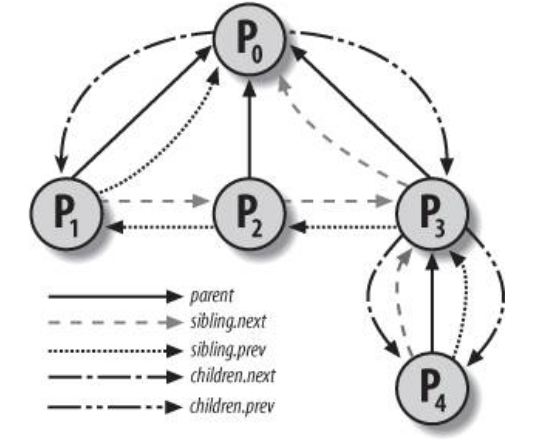
\includegraphics[width=0.7\textwidth]{parent2.png}
\begin{block}{思考}
给定指向某进程描述符的指针p, 如何打印该进程所有子进程的ID? (实现这个函数,可使用\verb|list_for_each|宏)
\end{block}
\end{frame}

\begin{frame}[fragile]
%\frametitle{Linux进程表示:task\_struct结构}
\frametitle{表示进程其他关系的字段}
进程标识:

\begin{itemize}
\item 从内核角度,一律通过task\_struct操作进程
\item 从用户角度可能需要通过PID操作进程,如kill(pid)
\end{itemize}

所以需要做到从pid到task\_struct的快速转换:

\begin{itemize}
\item task\_struct到pid: \verb|p->pid|
\item pid到task\_struct的快速转换:
\begin{itemize}
\item 遍历所有进程,逐一检查其pid字段的值?
\item 通过散列表结构做到快速转换
\end{itemize}
\item (重要)给定进程组、会话组或者线程组的leader ID, 如何快速找出该组中所有进程(线程)?
\end{itemize}

\end{frame}

\defverbatim[colored]\lstpidtype{
\begin{lstlisting}[tabsize=8,basicstyle=\ttfamily]
enum pid_type
{
    PIDTYPE_PID,
    PIDTYPE_TGID,
    PIDTYPE_PGID,
    PIDTYPE_SID,
    PIDTYPE_MAX
};
\end{lstlisting}
}
\defverbatim[colored]\lstpidhashhaha{
\begin{lstlisting}[tabsize=8,basicstyle=\ttfamily]
static struct hlist_head *pid_hash[PIDTYPE_MAX];
\end{lstlisting}
}
\begin{frame}[fragile]
\frametitle{表示进程其他关系的字段}
共有四种类型的PID:进程本身PID、线程组leader的PID、进程组leader的PID以及会话组leader的PID:
\begin{block}{include/linux/pid.h}
\lstpidtype
\end{block}
\end{frame}

\begin{frame}[fragile]
\frametitle{表示进程其他关系的字段}
\begin{block}{依据PID类型不同,共定义四个散列表:kernel/pid.c}
\lstpidhashhaha
\end{block}
\begin{block}{思考}
%\lstpidhashhaha
为什么定义这个数组时使用指向\verb|hlist_head|的指针?
\end{block}
\end{frame}

\defverbatim[colored]\lstpidstruct{
\begin{lstlisting}[tabsize=8,basicstyle=\ttfamily]
struct pid
{
    int nr;
    struct hlist_node pid_chain;
    struct list_head pid_list;
};
\end{lstlisting}
}
\defverbatim[colored]\lstpidsintaskstruct{
\begin{lstlisting}[tabsize=8,basicstyle=\ttfamily]
struct task_struct
{
    ...
    /* PID/PID hash table linkage. */
    struct pid pids[PIDTYPE_MAX];
    ...
};
\end{lstlisting}
}
\begin{frame}[fragile]
\frametitle{表示进程其他关系的字段}
\begin{block}{散列表中元素struct pid: include/linux/pid.h }
\lstpidstruct
\end{block}
\begin{block}{task\_struct中相应字段}
\lstpidsintaskstruct
\end{block}
\end{frame}

\defverbatim[colored]\lsthashfunction{
\begin{lstlisting}[tabsize=8,basicstyle=\ttfamily]
unsigned long hash_long(unsigned long val, unsigned int bits)
{
    unsigned long hash = val * 0x9e370001UL;
    return hash >> (32 - bits);
}
\end{lstlisting}
}
\begin{frame}[fragile]
\frametitle{表示进程其他关系的字段}
\begin{block}{哈希函数的定义}
\lsthashfunction
\end{block}
\begin{block}{思考}
\begin{itemize}
\item 这里的参数\verb|bits|起到什么作用? 
\item 对于含有2048个\verb|hlist_head|元素的散列表而言,参数\verb|bits|
应该是多少?
\end{itemize}
\end{block}
\end{frame}

\begin{frame}[fragile]
\frametitle{表示进程其他关系的字段: pid\_hash结构图} 
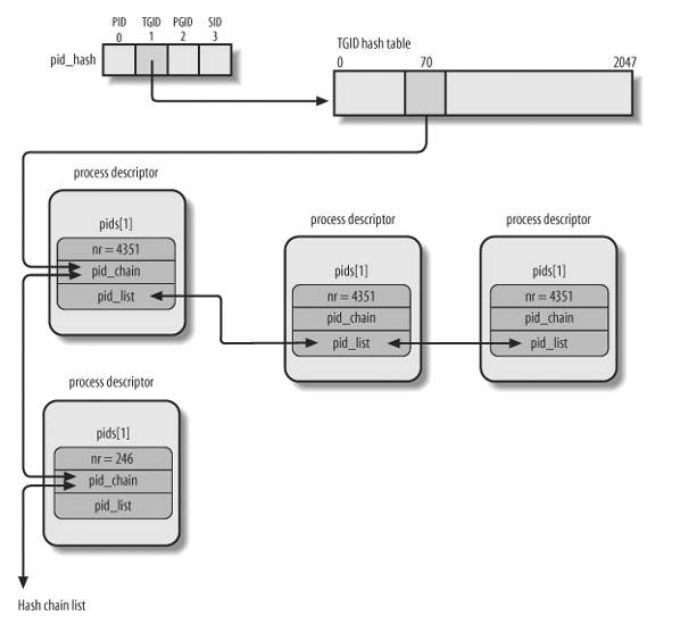
\includegraphics[width=0.7\textwidth]{pidhashes.png}
\begin{block}{考试要求}
能够根据这个数据结构图,描述如何从pid确定进程描述符的地址,以及如何根据pid及其类型,确定小组内全体成员。
\end{block}
\end{frame}

\begin{frame}[fragile]
\frametitle{Intel平台上的分页技术}
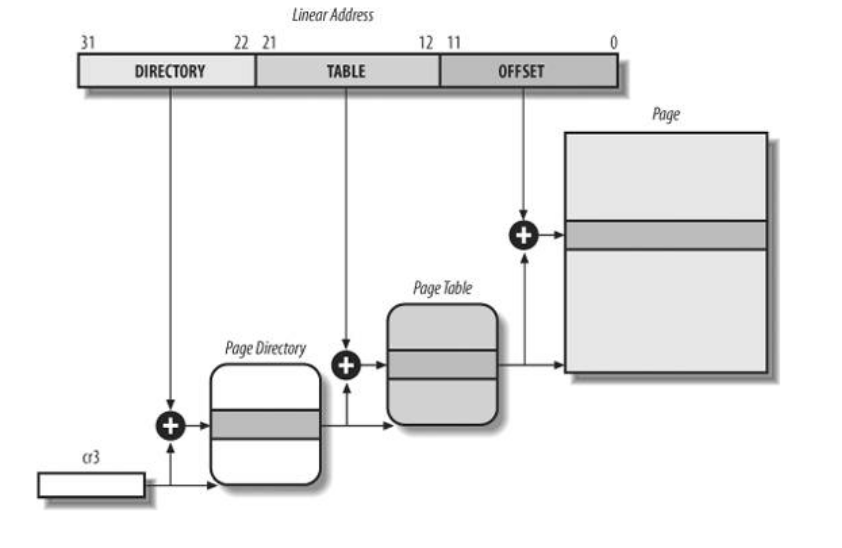
\includegraphics[width=0.8\textwidth]{regpaging.png}

cr3寄存器用于存放当前进程的page directory(第一级页表).
\end{frame}

\begin{frame}[fragile]
\frametitle{Intel平台上的扩展分页模式}
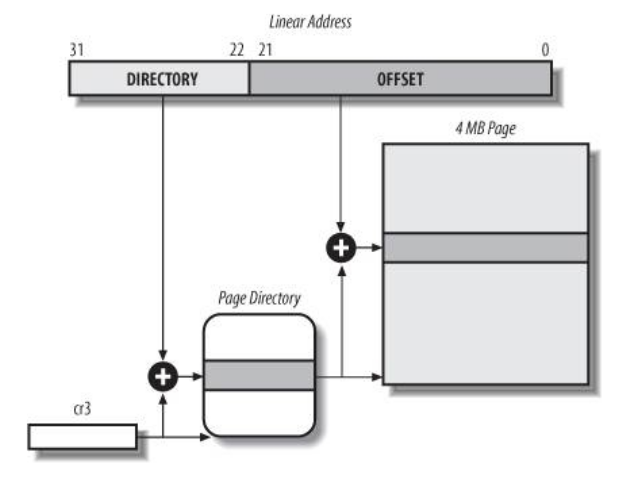
\includegraphics[width=0.8\textwidth]{extpaging.png}

扩展分页模式下,页面大小为4M,用于处理大块连续地址空间,
以节省页表所占空间及TLB空间。
\end{frame}

\begin{frame}[fragile]
\frametitle{分页的实际例子}
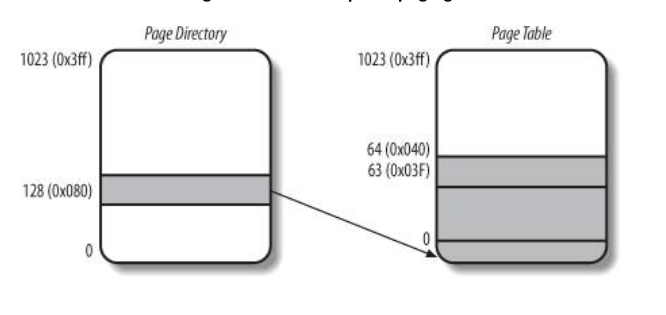
\includegraphics[width=0.8\textwidth]{examplepaging.png}

假设内核把从\verb|0x20000000|到\verb|0x2003ffff|之间的线性地址(共64页)分配给某进程。
\begin{itemize}
\item 该段地址最高10位均为\verb|0010000000|, 即\verb|0x080|(十进制128),因此第一级页表只有一个页表项有效。
\item 该段地址中间10位范围为0 -- \verb|0x03f|(即0 -- 63). 所以第二级页表中开头64个页表项有效。(图示灰色区域)
\item 给定线性地址\verb|0x20021406|,如何确定其对应的物理地址?
\end{itemize}

\end{frame}

\end{CJK*}
\end{document}
